\subsection{Filtrering}
Filtrering er et værktøj indenfor databehandling, som anvendes i det målte signals frekvensdomæne. Formålet med at filtrere et målt signal er at fjerne uønskede frekvenser, også kaldet støj, der ikke tilhører det signal der ønskes undersøgt. Filtret kan opdele signalet i såkaldte bånd: Pasbånd, hvor frekvenserne frit passerer igennem filteret uden påvirkning, samt stopbånd hvor frekvenserne dæmpes, så de ikke har indflydelse på signalet. Dette gøres ved en knækfrekvens.
Der findes flere forskellige typer af filtre, afhængigt af hvilke frekvenser der skal fjernes fra det målte signal \cite{Devasahayam2000}:

\begin{itemize}
	\item Lavpasfiltret anvendes til at dæmpe frekvenser over den valgte knækfrekvens. Dette gøres ved at dæmpe de frekvenser som ligger over knækfrekvensen.
	\item Højpasfilteret anvendes, modsat lavpasfiltret, til at dæmpe frekvenser under den valgte knækfrekvens, ved at dæmpe signalet under knækfrekvensen.
	\item Båndpasfilteret er en kombination af et lav- og højpasfilter.  Her defineres et interval, hvormed de frekvenser der ligger udenfor intervallet vil blive dæmpet.
	\item Båndstopfilteret fungerer modsat båndpasfilteret ved at dæmpe specifikt definerede frekvensområder. Frekvenserne udenfor det definerede område påvirkes ikke. 
\end{itemize}
  
Princippet i de fire filtertyper er illustreret på \fxnote{Referer til figur}.
\begin{figure}[H]
\centering
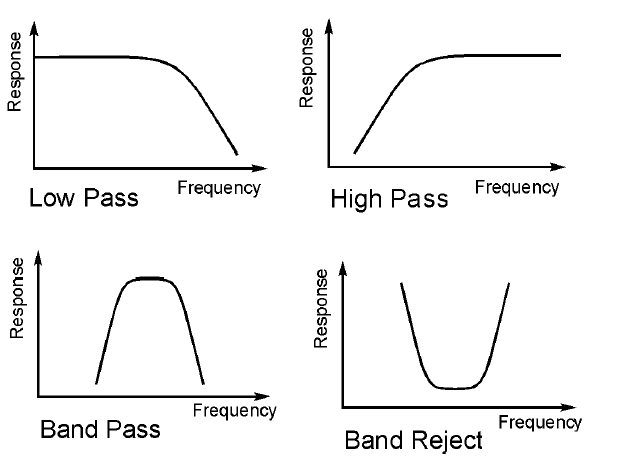
\includegraphics[scale=1.0]{figures/bproblemanalyse/filtertyper.png}
\caption{De fire filtertyper ses her \cite{2. semester kristian}}
\label{fig:filtertyper}
\end{figure}
I forbindelse med databehandling kan flere af filtrene anvendes samtidig. \cite{Devasahayam2000}

\subsubsection{Støj}
Støj er en uønsket del af et opsamlet signal, som ikke har nogen relation til det signal som ønskes målt\fxnote{Indsæt kilde}. Signaler der er fordelt udover et frekvensspektrum kan filtreres for støj vha. de tidligere beskrevne filtre. \cite{Devasahayam2000}
Støj kan inddeles i flere forskellige generelle typer, som typisk vil forekomme:

\textbf{Elektriske signaler} Dette er bl.a. 50 hz støj. 50 hz er den frekvens som elnettet vi har rundt omrking i vores dagligdag udsender. Denne 50 hz frekvens kan gå ind og påvirke de biologiske signaler som der måles på. Hvis der er flere 50 hz kilder der interagerer kan det give ekko ved ved eksempelvis 100 hz og 150 hz. Det er denne form for støj der gerne skulle undgås, når signalet skal anaylseres.

\textbf{Ledninger} kan fungere som antenner, der kan opfange 50 hz støj og andre former for støj. Dette vil være et større problem jo længere ledningerne er. Ledningerne bliver også påvirket af de magnetfelter de kommer i kontakt med, dette gælder også for jordens magnetfelt. Magneltfelterne kan inducere størm i ledningerne hvilket også vil medføre støj. For at kontrollere den støj som ledningerne opfanger snoes de, så de opfanger den samme støj.


 

%STØJ: SKRIVE OM STØJ GENERELT - 50HZ OG STØJ FRA LEDNINGER
%FIND FIGURER - KIG I DET GAMLE PROJEKT
% 
 
